% !TEX root = ../report.tex
\section{Architecture evaluation}
The architecture that is shown in the previous chapters needs to be evaluated. This is done with the ATAM method. ATAM stands for Architecture Trade-off Analysis Method. This evaluation method is used to determine if the system meets the requirements that are composed in chapter 3. ATAM identifies critical design decisions and verifies them against our key drivers. If the design decisions do not fulfill the key drivers, risks for the system will be inevitable. In order to terminate these risks, solutions are provided to deal with the risks. In the remainder of this chapter the architectural approaches, utility tree and the scenarios are provided. 


% The ATAM method is used to evaluate the software architecture. The purpose of ATAM is elicit and refine a precise statement of the architecture’s driving quality attribute requirements\\
% • elicit and refine a precise statement of the architectural design decisions \\
% • evaluate the architectural design decisions to determine if they satisfactorily address the
% quality requirements [add source]
% %/ source: Using the Architecture Tradeoff Analysis Method to Evaluate a Wargame Simulation System: A Case Study Lawrence G. Jones Anthony J. Lattanze December 2001 Architecture Tradeoff Analysis Initiative 

% The method consists of the following steps:[add source] \\
% 1. Present the ATAM: The evaluation team presents a quick overview of the ATAM steps,
% techniques used, and outputs from the process. \\
% 2. Present the business drivers: The system manager briefly presents the business drivers
% and context for the architecture. \\
% 3. Present the architecture: The architect presents an overview of the architecture.
% 4. Identify architectural approaches: Itemize the architectural decisions discovered in the
% previous step.\\
% 5. Generate the quality attribute utility tree: Identify, prioritize, and refine the most
% important quality attribute goals in a utility tree format.\\
% 6. Analyze architectural approaches: Probe the architectural approaches in light of the
% quality attributes in order to identify risks, sensitivity points, and tradeoffs.\\
% 7. Brainstorm and prioritize scenarios: Create and analyze scenarios that represent the
% various stakeholders’ interests to understand quality attribute requirements and their
% relative importance.\\
% 8. Analyze architectural approaches: Continue to identify risks, sensitivity points, and
% tradeoffs while noting the impact of each scenario on the architectural approaches. \\
% 9. Present results: Recapitulate the ATAM steps, outputs, and recommendations. \\
% %/ source: Using the Architecture Tradeoff Analysis Method to Evaluate a Wargame Simulation System: A Case Study Lawrence G. Jones Anthony J. Lattanze December 2001 Architecture Tradeoff Analysis Initiative 

% The first three steps are presented in the previous chapters. In this sub-chapter the focus will be on step 4 and further. 

\subsection{Architectural approaches}
This section lists the architectural approaches used in the document.
The most important part of our system is to warn people in case of a flood. The decision was made to warn citizens through SMS. This solution is available for all mobile phones and can used without the use of internet. It is the most reliable solution to warn citizens. To warn the safety region, the decision was made to use the emergency room API. This API is able to receive warnings and updates from our system. 

Another major design decision was how to connect the different sensors to the system. The decision was made to use a wired connection between the sensors and the hubs. A wireless protocol wouldn't suffice, since the signal isn't strong enough to go through dikes. Connecting sensors to the hubs in this way, makes it also easier to power the sensors. A power wire can simply be added, instead of using batteries or solar panels. The decision to use hubs was made to make the system more structured and organised. Hubs can send data to the central system, this means the system doesn't get to much connections. 

Citizens want to get proper guidance in case of a flood. Third party developers will develop this feature. In order to make this happen the system provides data to the third party developers. The decision to let third party developers develop this application was chosen over developing such a feature ourselves. This was done to keep the focus fully at designing a good architecture for the most important part, the flood detecting and warning system. This decision also gives the possibility for other developers to use our data and create creative applications. 

In the software architecture, the layer pattern is used to seperate the functionality of the system. This is implemented to make the system more reliable, maintainable and extendable.

Short summary of the most important decisions:
\begin{itemize}
	\item Send warnings by SMS to citizens
	\item Use the emergency room API to warn the safety region
	\item Use hubs to connect the sensors to the system
	\item Connect sensors through wires to the hubs
	\item Allow third party developers to create a guidance application
	\item Use the layer pattern in the software architecture
\end{itemize}


\subsection{Quality attribute utility tree approaches}
The utility tree is one of the ATAM techniques it represents the overall usefulness of the system. 
In this section the utility tree is built according to the key drivers of our system : reliability, performance and availability ( view part 3.3 ). The purpose of the utility tree is to elect high priority scenarios which will be analysed precisely in the next section.
The scenarios serve as the leafs of the utility tree and the architecture is evaluated by considering how it makes the scenarios possible. \\


There are four levels in the three . The first node is the root : " Utility " , then follow the Quality factors which are our key drivers , then the tree goes deeper in precision with refined the key drivers in subfactors which are demonstrated by the leaves with the scenarios we expect our system to manifest. \\

In order to prioritize the scenarios two criterias are used and classified as follow: \\
\textit{Importance  to system success}: High (Very important feature for the system : essential), Medium, Low (Not mandatory)\\
\textit{ Risk/difficulty in achieving}: High, Medium, Low\\
To get the meaning of High , Medium and Low we can use a scale from 10 to 0 as reference: High : 10-7, Medium 6-4, Low 4-0.

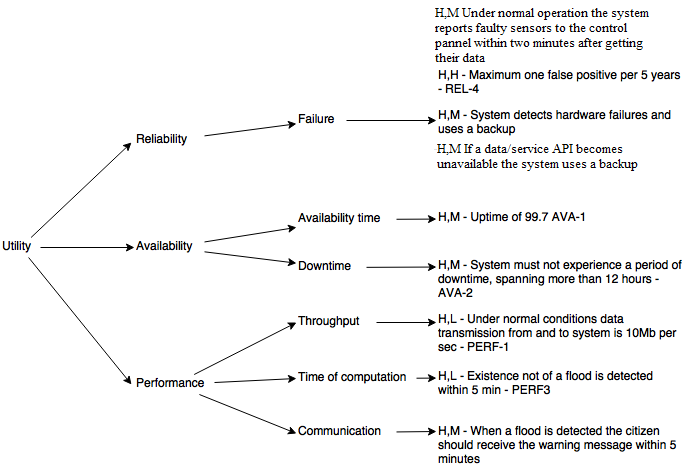
\includegraphics[scale=0.8]{images/utilitytree1.png}

The interesting scenarios are the ones with high priority (H,H),(H,M) and (M,H), focus will be put on them in the next section.

\subsection{Scenarios}

In this part high priority scenarios derived from the utility tree will be analysed and as a result will come the identification of sensitivity points, tradeoffs, risks and non risks.


% From reading material:
% Risks are potentially problematic architectural decisions. 
% Non-risks are good decisions that rely on assumptions that are frequently implicit in the architecture.

\begin{table}[H]
	\begin{tabular}{L{0.2\textwidth} L{0.6\textwidth}}
		\textbf{Scenario}		& \textbf{Handling faulty sensors} \\ \toprule
		\textbf{Q-Attribute(s)} & Availability, reliability \\ \midrule
		\textbf{Environment} 	& Normal operation \\ \midrule
		\textbf{Stimulus} 		& A sensor sends wrong data or stops sending data \\ \midrule
		\textbf{Response} 		& The system ignores the sensor until is has been repaired/replaced \\ \midrule
		\textbf{Design decisions} 	& \\
			\multicolumn{2}{c}{
			\begin{tabular}{l|lllll}
				\textbf{Decision} & Req. & Sensitiv. & Tradeoff & Risk & Non-Risk \\ \hline
				
				Detection algorithm & \ref{fr:detect-faultysensor}, \ref{rel:2} & \nsl{s}{faultysensor} & \nsl{to}{faultysensor} &  & \nsl{nr}{detection}  \\
				Reporting & \ref{fr:report-faultysensors} &  &  & \nsl{r}{reportfaultysensor} &  \\
				UAV & \ref{fr:uav} & \nsl{s}{uav} & \nsl{to}{uav} & \nsl{r}{uav-weather} & \\
				
			\end{tabular} 
			} \\
			\midrule
			\multicolumn{2}{c}{\compactCell{
				\textbf{Sensitivities:} 
				\begin{itemize} \setlength{\itemsep}{-15pt}
				\item \ref{s:faultysensor}: Some of the time, it will be difficult for the detection algorithm to distinguish between extreme data from a sensor caused by a fault and extreme data caused by a flood.\\
				\item \ref{s:uav}: It takes time for the UAV to be dispatched to the potential flood location.
				\end{itemize} ~\\[-0.5cm]
				\textbf{Tradeoffs:} 
				\begin{itemize} \setlength{\itemsep}{-15pt}
				\item \ref{to:faultysensor}: Reliability (+) vs. Performance (-) -- Using an algorithm on the sensor data to detect faulty sensors adds more overhead, but increases the reliability of the system.\\
				\item \ref{to:uav}: Reliability (+) vs. Performance (-) -- The UAV checks if a flood is present/developing when the sensor data is not conclusive. It has a large dispatch time, which means (if there is a flood), it will be detected with a larger delay. 
				\end{itemize} ~\\[-0.5cm]
				\textbf{Risks:} 
				\begin{itemize} \setlength{\itemsep}{-3pt}
				\item \ref{r:reportfaultysensor}: There is a risk that the config panel where the faulty sensors are reported, is not checked often enough, leading to broken sensors not being replaced. See \ref{risk:configpanel-notchecked}.
				\item \ref{r:uav-weather}: There is a risk that the weather will not allow the UAV to fly. See \ref{risk:uav-badweather}.
				\end{itemize}
				\textbf{Non-Risks:} 
				\begin{itemize} \setlength{\itemsep}{-3pt}
					\item \ref{nr:detection}: The presence of a detection algorithm will increase reliability, since it will filter faulty sensor data
				\end{itemize}
			}} \\

		\midrule
		\textbf{Reasoning} 		& Temporarily ignoring faulty sensors allows the system to continue functioning. Reporting the sensors using the control panel allows maintenance personnel to repair those sensors. It is important that maintenance personnel checks the control panel regularly. 
		
		In case it cannot be determined by the system if a sensor is faulty, or whether there is a flood, a UAV can be dispatched to check. \\
		%\midrule
		%\textbf{Arch. model} 	&  \\
								 
	 \bottomrule
	\end{tabular}
	\label{ATAM:faulty-sensors}
	\caption{ATAM -- Handling faulty sensors}
\end{table}

\begin{table}[H]
	\begin{tabular}{L{0.2\textwidth} L{0.6\textwidth}}
		\textbf{Scenario}		& \textbf{Handling hardware failures} \\ \toprule
		\textbf{Q-Attribute(s)} & Availability \\ \midrule
		\textbf{Environment} 	& Normal operation \\ \midrule
		\textbf{Stimulus} 		& A hardware component stops operating \\ \midrule
		\textbf{Response} 		& The system uses a backup of the hardware component \\ \midrule
		\textbf{Design decisions} 	& \\
			\multicolumn{2}{c}{
			\begin{tabular}{l|lllll}
				\textbf{Decision} & Req. & Sensitiv. & Tradeoff & Risk & Non-Risk \\ \hline
				
				Database cluster & \ref{ava:1}, \ref{ava:2} &  & \nsl{to}{cluster} &  & \nsl{nr}{clusterdb}  \\
				Analytic cluster & \ref{ava:1}, \ref{ava:2} &  & \ref{to:cluster} &  & \nsl{nr}{clusteranalytic} \\
				Multiple data centers & \ref{ava:1}, \ref{ava:2} &  & \nsl{to}{datacentre} &  & \nsl{nr}{datacenters} \\
				Arduino               & \ref{ava:1}, \ref{ava:2} & \nsl{s}{arduinofail} &  & \nsl{r}{arduinofail} &  \\
				
			\end{tabular} 
			} \\
			\midrule
			\multicolumn{2}{c}{\compactCell{
				\textbf{Sensitivities:} 
				\begin{itemize} \setlength{\itemsep}{-15pt}
				\item \ref{s:arduinofail}: The Arduino are hardware components which can fail as well. Several sensors are connected to a single Arduino. Since a failing Arduino does not have a backup, those sensors connected to it will become unavailable to the system until the Arduino is repaired. \\
				\end{itemize} ~\\[-1.0cm]
				\textbf{Tradeoffs:} 
				\begin{itemize} \setlength{\itemsep}{-15pt}
				\item \ref{to:cluster}: Availability (+) vs. Affordability (-) -- Using a cluster is more expensive, but provides a fallback in case of failures, increasing the availability. \\
				\item \ref{to:datacentre}: Also Availability (+) vs Affordability (-) -- The costs of the system increase significantly by having a second data center. However, this guarantees the availability of the system in case of problems with one of the data centers.
				\end{itemize} ~\\[-0.5cm]
				\textbf{Risks}
				\begin{itemize}
				\item \ref{r:arduinofail}: Since only one Arduino is used to connect several sensors, the Arduino going offline will mean that multiple sensor become detached from the system. See \ref{risk:arduino-broken}.
				\end{itemize}
				
				\textbf{Non-Risks:} 
				\begin{itemize} \setlength{\itemsep}{-3pt}
				\item \ref{nr:datacenters}: Multiple data centers aid with increasing the availability only when they are not placed in close proximity to each other.
				\item \ref{nr:clusterdb}: The database cluster will be configured for replication, which means the availability of the data is guaranteed
				\item \ref{nr:clusteranalytic}: Using a cluster for the analytics will assure not only availability of the analytic component, but also increase the performance, since the computational load is divided amongst multiple analytic nodes
				\end{itemize}
			}} \\

		\midrule
		\textbf{Reasoning} 		& The hardware in the data centers and the data center itself are prepared for failures of components. It is important to note that the data centers should not be placed in close proximity to each other. 
		
		A failure of an Arduino will lead to several sensors going offline, but these sensor are located in a relatively small area and therefore only have a limited impact on the systems monitoring capabilities. \\
		\midrule
		\textbf{Arch. model} 	& See figure~\ref{fig:database-cluster} and figure~\ref{fig:analytic-cluster} for the logical schematic of the database and analytic cluster respectively.
		
		Also see figure~\ref{fig:hardware-archi-schema} for an overview of the multiple data centers. \\
								 
	 \bottomrule
	\end{tabular}
	\caption{ATAM -- Handling hardware failures}
	\label{ATAM:hardware-failure}
\end{table}

\begin{table}[H]
	\begin{tabular}{L{0.2\textwidth} L{0.6\textwidth}}
		\textbf{Scenario}		& \textbf{Ensuring availability of third party data / services} \\ \toprule
		\textbf{Q-Attribute(s)} & Availability, reliability, interoperability \\ \midrule
		\textbf{Environment} 	& Normal operation \\ \midrule
		\textbf{Stimulus} 		& A third party service or data API becomes unavailable \\ \midrule
		\textbf{Response} 		& The system still has access to (a backup of) the data or service \\ \midrule
		\textbf{Design decisions} 	& \\
			\multicolumn{2}{c}{
			\begin{tabular}{l|lllll}
				\textbf{Decision} & Req. & Sensitiv. & Tradeoff & Risk & Non-Risk \\ \hline
				
				Using multiple API providers offering same service/data & \ref{fr:receive-weather}, \ref{fr:receive-geographic} &  & \nsl{to}{apis} &  & \nsl{nr}{multipleapi}  \\
				SMS service & \ref{fr:warn-citizens}, \ref{fr:citizens-subscribe} & \nsl{s}{onesmsservice} &  & \nsl{r}{sms} & \nsl{nr}{storingphonenrs}  \\
				Emergency room API & \ref{fr:warn-safetyregion} &  &  &  &  \nsl{nr}{emergencyroomapi} \\
				
				
			\end{tabular} 
			} \\
			\midrule
			\multicolumn{2}{c}{\compactCell{
				\textbf{Sensitivities:} 
				\begin{itemize} \setlength{\itemsep}{-15pt}
				\item \ref{s:onesmsservice}: The system relies on a single SMS Service provider (CM Telecom). If this provider is not available, the system cannot warn citizens by text message. \\
				\end{itemize} ~\\[-1.0cm]
				\textbf{Tradeoffs:} 
				\begin{itemize} \setlength{\itemsep}{-15pt}
				\item \ref{to:apis}: Reliability (+) vs. Affordability (-) -- Most APIs charge a usage fee, which means that using multiple APIs increases the costs. \\
				\end{itemize} ~\\[-1.0cm]
				\textbf{Risks:} 
				\begin{itemize} \setlength{\itemsep}{-3pt}
				\item \ref{r:sms}: Since the system depends on a single SMS Service, if this SMS service goes offline, it cannot be used to warn the citizens. See \ref{risk:sms-service-online}.
				\end{itemize}
				\textbf{Non-Risks:} 
				\begin{itemize} \setlength{\itemsep}{-3pt}
				\item \ref{nr:storingphonenrs}: The phone numbers of citizens who subscribed are stored in the database of the system instead of the SMS Service provider's database.
				\item \ref{nr:emergencyroomapi}: It is assumed that the emergency room API is always available, which is the responsibility of the safety region.
				\item \ref{nr:multipleapi}: Using multiple APIs for the external data services allows access to such data if one of the APIs are offline.
				\end{itemize}
			}} \\

		\midrule
		\textbf{Reasoning} 		& \compactCell{
			By using multiple APIs for weather / geographic / demographic data, it is ensured that this data is available if one of the APIs goes offline. 
			
			The SMS service is a single point of failure: if it goes offline, there is no backup SMS service provider.
		} \\
		%\midrule
		%\textbf{Arch. model} 	& \\
								 
	 \bottomrule
	\end{tabular}
	\caption{ATAM -- Ensuring availability of third party data / services}
	\label{ATAM:3rdpartydata}
\end{table}
